\documentclass{beamer}

\title{Modelos Generativos Profundos}
\subtitle{Clase 7: Modelos autorregresivos y LLMs (parte III)}
\author{Fernando Fêtis Riquelme}
\institute{
    Facultad de Ciencias Físicas y Matemáticas\\
    Universidad de Chile
}
\date{Otoño, 2026}
\titlegraphic{\hfill
\includegraphics[height=1.2cm]{images/fcfm}}

\usetheme{metropolis}
\setbeamercovered{transparent}

\newcommand{\R}{\mathbb{R}}
\newcommand{\N}{\mathbb{N}}
\newcommand{\Z}{\mathbb{Z}}
\newcommand{\argmax}{\operatorname{argmax}}
\newcommand{\insertimage}[2]{
    \begin{center}
        \includegraphics[width=#2\textwidth]{images/#1}
    \end{center}
}
\renewcommand{\raggedright}{\leftskip=0pt \rightskip=0pt plus 0cm}
\setlength{\leftmargini}{0em}

\begin{document}

\begin{frame}
    \titlepage
\end{frame}

\begin{frame}{Clase de hoy}
    \tableofcontents
\end{frame}

\begin{frame}{Introducción}
    En la clase anterior se estudió la arquitectura GPT, la cual permite entender el esqueleto general que siguen los modelos autorregresivos actuales.

    Si bien este esqueleto general se ha mantenido a lo largo del tiempo, se han introducido muchas modificaciones a la arquitectura original, las cuales han permitido mejorar la eficiencia y rendimiento de los modelos.

    Más aún, los LLMs solo son una aplicación de la arquitectura Transformer, la cual hoy en día se utiliza de manera transversal en el machine learning moderno.

    En esta clase se revisarán algunas variaciones usuales de los componentes que constituyen la arquitectura Transformer.
\end{frame}

\section{Tokenizadores}

\begin{frame}{Problema de tokenización}
    Dado un dominio de texto, es necesario elegir un \textbf{algoritmo de tokenización}, el cual definirá el vocabulario $\mathcal{V}$ sobre el que se tokenizará dicho corpus.
    \begin{itemize}
        \item Aumentar $|\mathcal{V}|$ aumenta la cantidad de parámetros del modelo.
        \item Disminuir $|\mathcal{V}|$ provoca que las secuencias de tokens sean más largas, lo cual aumenta el costo de procesamiento.
    \end{itemize}
    Encontrar la \textit{mejor} tokenización es un problema NP-completo, por lo que se debe recurrir a métodos aproximados.
\end{frame}

\begin{frame}{Byte pair encoding}
    Uno de los algoritmos de tokenización más usuales es el algoritmo \textbf{byte pair encoding (BPE)}:
    \begin{itemize}
        \item Comienza considerando cada caracter como un token de $\mathcal{V}$.
        \item Luego, forma nuevos tokens combinando cadenas de caracteres de acuerdo a su frecuencia de ocurrencia en el corpus.
        \item Para esto, calcula la frecuencia de todos los bigramas en el corpus y agrega al vocabulario el bigrama con mayor frecuencia.
        \item Este proceso se repite hasta que se alcanza el tamaño de vocabulario deseado.
        \item Otros algoritmos como \textbf{WordPiece} siguen enfoques similares.
    \end{itemize}
\end{frame}

\begin{frame}{Tokens especiales}
    Es usual incluir \textbf{tokens especiales} que cumplen funciones específicas en el modelo. Algunos ejemplos son:
    \begin{itemize}
        \item \textbf{$\text{<SEP>}$:} usado para separar dos partes de la secuencia.
        \item \textbf{$\text{<CLS>}$:} usado como embedding de la secuencia completa.
        \item \textbf{$\text{<MASK>}$:} usado para enmascarar partes de la secuencia.
        \item \textbf{$\text{<TOOL>}$:} usado para demarcar el uso de herramientas externas.
        \item \textbf{$\text{<SYSTEM>}$, $\text{<USER>}$, $\text{<ASSISTANT>}$:} usado para indicar roles dentro de una conversación.
        \item \textbf{$\text{<THINKING>}$:} usado para demarcar el proceso de razonamiento interno del modelo.
    \end{itemize}
\end{frame}

\section{Positional encoding}

\begin{frame}{Motivación}
    Omitiendo el masking causal aplicado en el mecanismo de self-attention, un bloque Transformer es \textbf{equivariante bajo permutaciones}. Es decir, para una entrada $(x_1,\ldots,x_T)$:
    \begin{equation*}
        \text{Transformer}(\sigma(x_1,\ldots,x_T)) = \sigma(\text{Transformer}(x_1,\ldots,x_T)),
    \end{equation*}
    para toda permutación $\sigma:\{1,\ldots,T\}\to\{1,\ldots,T\}$.

    En consecuencia, es necesario inyectar información posicional a la arquitectura para que esta pueda conocer el orden de los tokens dentro de la secuencia y no actúe simplemente como una \textbf{bag of embeddings}.
\end{frame}

\begin{frame}{Embeddings posicionales absolutos}
    Una forma sencilla de inyectar información posicional es utilizando una capa de \textbf{embedding posicional absoluto} (APE), la cual asigna a cada posición $t\in\{1,\ldots,T\}$ un vector de embedding $p_t\in\R^D$.

    De esta forma, en lugar de alimentar el bloque Transformer con la secuencia de embeddings $(x_1,\ldots,x_T)$, se alimenta con la secuencia $(x_1+p_1,\ldots,x_T+p_T)$.

    Dado que una capa de embedding es una lookup table entrenable, esta técnica restringe la longitud máxima de las secuencias a un valor predefinido, $T_{\max}\in\N$, conocido como \textbf{ventana de contexto}.
\end{frame}

\begin{frame}{Embeddings posicionales sinusoidales}
    Otra opción para APEs es utilizar \textbf{embeddings sinusoidales}:
    \begin{equation*}
        p_t=
        \left(
        \begin{matrix}
                \sin(\omega_1 t) \\ \cos(\omega_1 t)\\ \vdots \\ \sin(\omega_{D/2} t)\\ \cos(\omega_{D/2} t)
            \end{matrix}
        \right)\in[-1,1]^D
    \end{equation*}
    \vspace{-0.5cm}
    \begin{itemize}
        \item Las \textbf{frecuencias de oscilación}, $\omega_1,\ldots,\omega_{D/2}>0$, suelen elegirse siguiendo una progresión geométrica decreciente.
        \item Es decir, $\omega_k = b^{-\frac{k}{D}}$, donde $b>1$ es un hiperparámetro.
        \item Notar que este mecanismo no utiliza parámetros entrenables.
    \end{itemize}
\end{frame}

\begin{frame}{Embeddings posicionales sinusoidales}
    \insertimage{sinusoidal}{0.8}
\end{frame}

\begin{frame}{Embeddings posicionales relativos}
    Una posible variación de los APEs es utilizar \textbf{embeddings posicionales relativos} (RPE), los cuales, en vez de asignar un embedding a cada posición, asignan un embedding a cada posible distancia entre posiciones.

    Para esto, notar que el único lugar donde interactúan los embeddings de distintas posiciones dentro de un bloque Transformer es el mecanismo de atención.

    Si bien se han propuesto muchas formas de implementar RPEs, se revisarán dos de las más usuales:
    \begin{itemize}
        \item \textbf{Attention with linear biases (ALiBi)}.
        \item \textbf{Rotary positional embeddings (RoPE)}.
    \end{itemize}
\end{frame}

\begin{frame}{Attention with linear biases}
    En el mecanismo de atención usual, se calculan los scores de atención como $s_{ij}=\frac{\langle q_i, k_j\rangle}{\sqrt{P}}$.

    ALiBi modifica esta fórmula para incluir información posicional relativa:
    \begin{equation*}
        s_{ij}=\frac{\langle q_i, k_j\rangle}{\sqrt{P}} + m|i-j|,
    \end{equation*}
    donde $m>0$ (\textbf{pendiente de sesgo}) es un hiperparámetro definido para cada cabezal de atención, provocando un trade-off entre atención global y local.
\end{frame}

\begin{frame}{Rotary positional embeddings}
    RoPE es un mecanismo de RPE que busca que el producto de atención solo dependa de los embedding $x_i$ y $x_j$, y de la distancia $i-j$.

    Es decir, busca funciones $f_q, f_k:\R^D\times\N\to\R^D$ para definir los vectores query y key como
    \begin{equation*}
        \begin{cases}
            q_i = f_q(x_i, i) \\
            k_j = f_k(x_j, j)
        \end{cases},
    \end{equation*}
    de modo que el producto de atención se pueda escribir como
    \begin{equation*}
        \langle q_i, k_j\rangle = g(x_i, x_j, i-j),
    \end{equation*}
    para alguna función $g:\R^D\times\R^D\times\Z\to\R$.
\end{frame}

\begin{frame}{Rotary positional embeddings}
    Una solución para este problema es definir $f_q$ y $f_k$ como rotaciones de los embeddings $x_i$ y $x_j$ respectivamente, donde el ángulo de rotación depende de la posición del token:
    \begin{equation*}
        f_{\{q,k\}}(x_k, k) = R_\Theta(k)W_{\{q,k\}}x_k,
    \end{equation*}
    donde $R_\Theta(k)\in\mathcal{M}_{D,D}(\R)$ es una matriz de rotaciones.

    De este modo, el producto de atención se puede escribir como
    \begin{equation*}
        \langle q_i, k_j\rangle = (W_q x_i)^\top R_\Theta(i-j) W_k x_j,
    \end{equation*}
    lo que cumple la condición deseada.
\end{frame}

\begin{frame}{Rotary positional embeddings}
    Para un conjunto de frecuencias $\Theta=\{\theta_1,\ldots,\theta_{D/2}\}$, la matriz de rotación $R_\Theta(k)\in\mathcal{M}_{D,D}(\R)$ de RoPE es una matriz bloque-diagonal, donde cada bloque es una matriz de rotación 2D con ángulo $k\theta_d$:
    \begin{equation*}
        R_\Theta(k) = \begin{pmatrix}
            \cos(k\theta_1) & -\sin(k\theta_1) & \cdots & 0                   & 0                    \\
            \sin(k\theta_1) & \cos(k\theta_1)  & \cdots & 0                   & 0                    \\
            \vdots          & \vdots           & \ddots & \vdots              & \vdots               \\
            0               & 0                & \cdots & \cos(k\theta_{D/2}) & -\sin(k\theta_{D/2}) \\
            0               & 0                & \cdots & \sin(k\theta_{D/2}) & \cos(k\theta_{D/2})
        \end{pmatrix}
    \end{equation*}
\end{frame}

\begin{frame}{No positional encoding (NoPE)}
    Por otro lado, si bien un bloque Transformer es equivarente bajo permutaciones, resulta ser que el mecanismo de masking causal sí inyecta información posicional implícita:
    \begin{figure}
        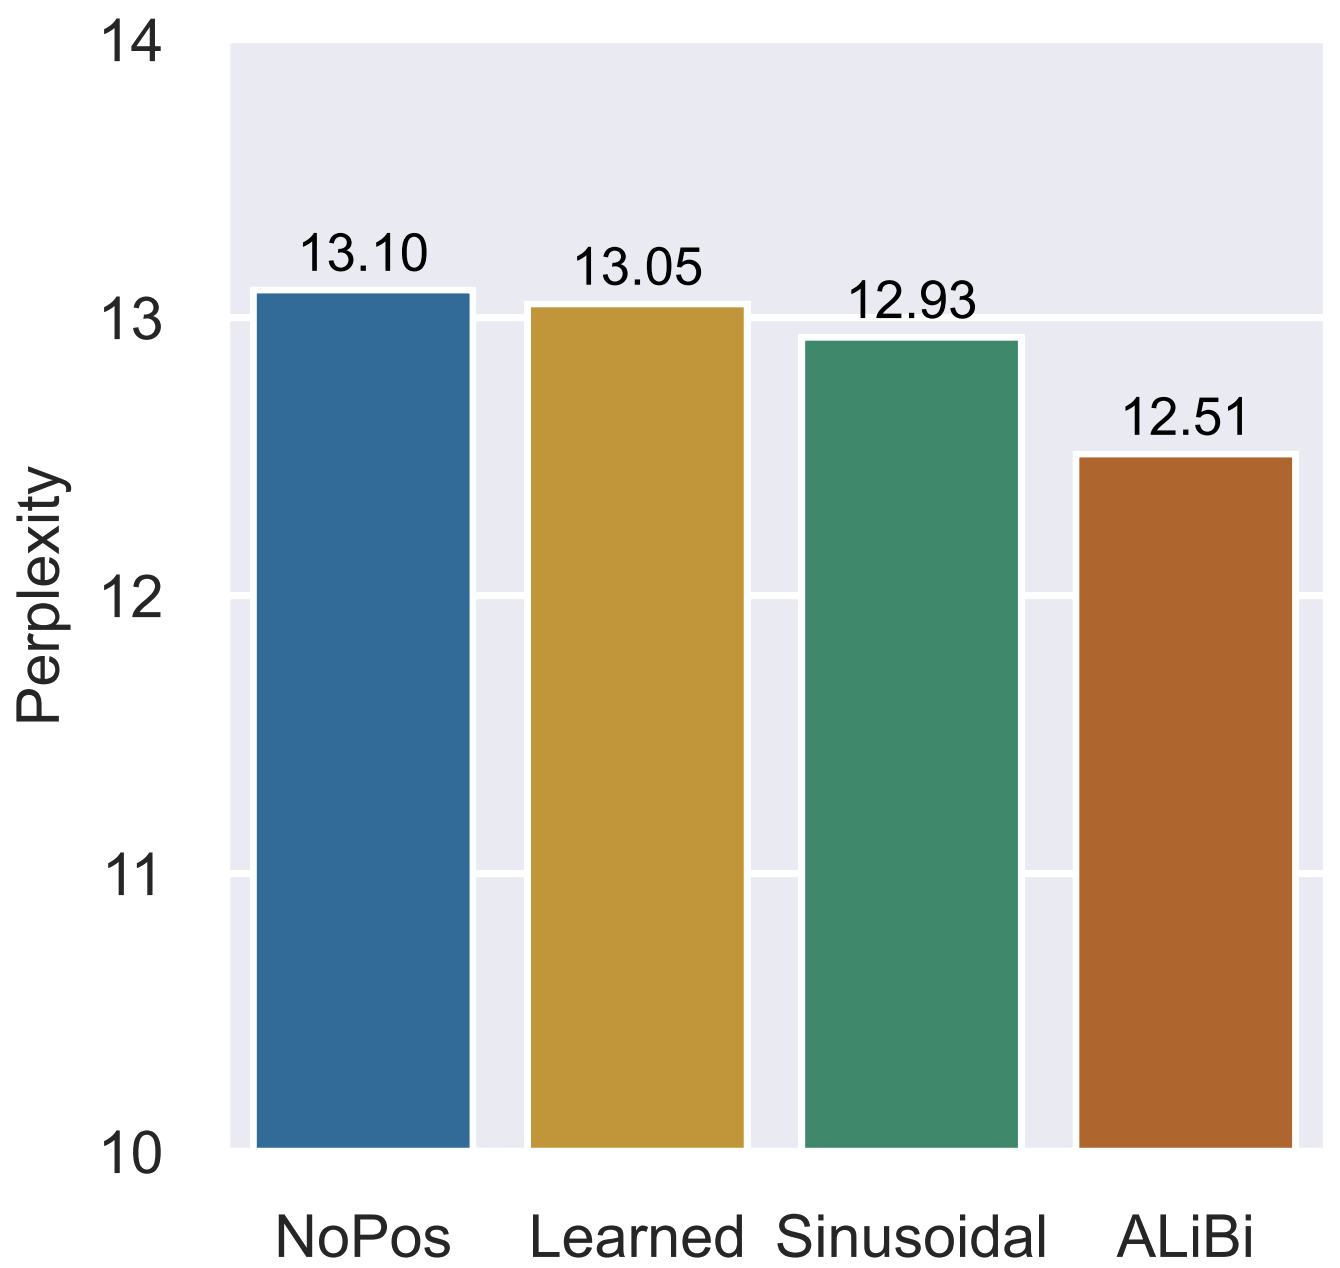
\includegraphics[height=0.45\textwidth]{images/nope1.png}
        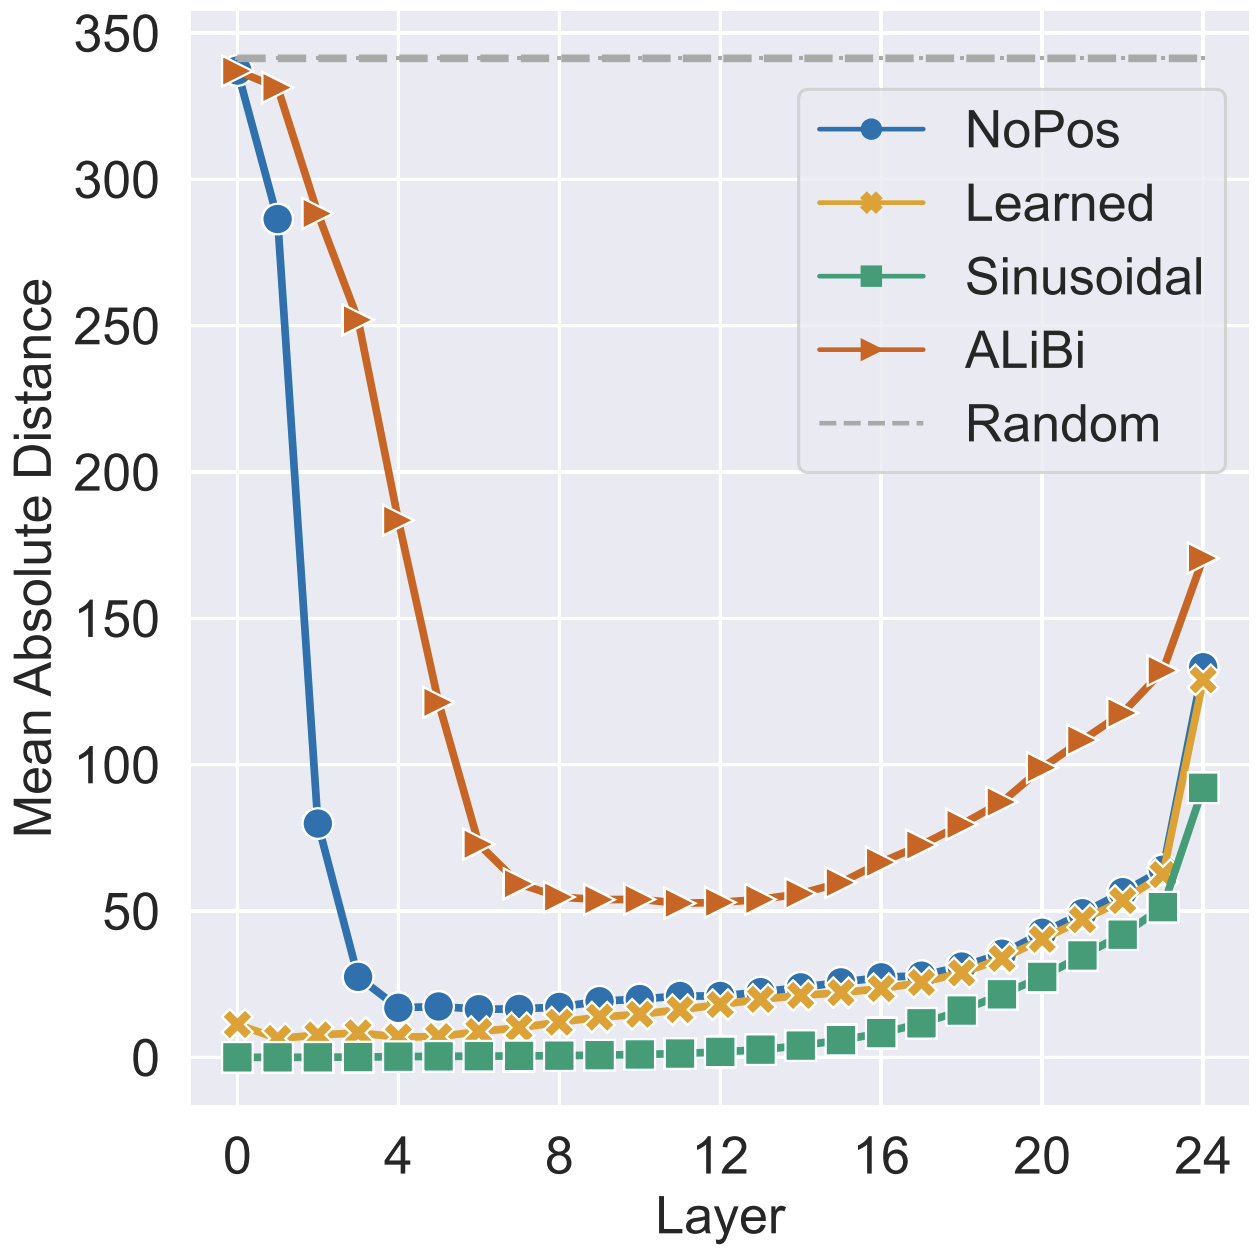
\includegraphics[height=0.45\textwidth]{images/nope2.png}
    \end{figure}
\end{frame}

\section{Mecanismos de normalización}

\begin{frame}{Capas de normalización}
    Una de las principales innovaciones que permitió entrenar CNNs profundas fue el uso de \textbf{batch normalization}.

    En el caso de modelos tipo GPT, los cuales también están formados por varias capas neuronales, también es necesario agregar capas de normalización.

    En este caso, es usual normalizar cada token de manera individual (i.e., sin considerar otros tokens u otras secuencias). Las dos alternativas más frecuentes son:
    \begin{itemize}
        \item \textbf{Layer normalization (LN)}.
        \item \textbf{Root mean square layer normalization (RMSNorm)}.
    \end{itemize}
\end{frame}

\begin{frame}{Layer normalization}
    \textbf{Layer normalization} normaliza (en media y varianza) cada vector de embedding individualmente:
    \begin{equation*}
        \text{LayerNorm}(x) := \alpha \odot \tilde{x} + \beta,
        \quad\text{donde}\quad
        \tilde{x} = \frac{x - \text{mean}(x)}{\text{std}(x)}
    \end{equation*}
    La ubicación de esta normalización dentro de los bloques MHSA y FF influye en la estabilidad del entrenamiento:
    \begin{itemize}
        \item \textbf{Post-LN:} es de la forma $x\mapsto\text{LayerNorm}(x+\text{SubLayer}(x))$
        \item \textbf{Pre-LN:} es de la forma $x\mapsto x+\text{SubLayer}(\text{LayerNorm}(x))$
    \end{itemize}
    Hoy en día se prefiere la arquitectura Pre-LN ya que genera una dinámica de entrenamiento más estable.
\end{frame}

\begin{frame}{Mecanismos de normalización}
    Otra técnica de normalización usual es \textbf{RMS normalization}, la cual calcula, para cada vector de embedding $x\in\R^D$:
    \begin{equation*}
        \text{RMSNorm}(x) = \alpha \odot \frac{x}{\text{rms}(x)},
        \quad\text{donde}\quad
        \text{rms}(x) = \sqrt{\frac{1}{D}\sum_{i=1}^{D} x_i^2}
    \end{equation*}
    \vspace{-0.5cm}
    \begin{itemize}
        \item Notar que $ \alpha \in \mathbb{R}^{D} $ es el único parámetro entrenable.
        \item RMSNorm normaliza todos los embeddings a una misma esfera de radio $\frac{1}{\sqrt{D}}$, la cual luego puede deformarse gracias al parámetro de escala $\alpha\in\R^D$.
        \item Este método de normalización se ha vuelto usual debido a que se puede computar eficientemente.
    \end{itemize}
\end{frame}

\section{Mecanismos de atención}

\begin{frame}{Atención aditiva y multiplicativa}
    Dada la importancia del mecanismo de atención, encontrar otras maneras definirlo puede mejorar considerablemente la eficiencia y rendimiento de un modelo.

    Para un vector query $q_i\in\R^P$ y un vector key $k_j\in\R^P$, se podría definir el score de atención, $s_{ij}\in\R$, de dos formas naturales:
    \begin{itemize}
        \item \textbf{Atención aditiva (Badhanau):} $s_{ij}=W_0\tanh\left(W_1q_i+W_2k_j\right)$.
        \item \textbf{Atención multiplicativa:} $s_{ij}=q_i^\top W k_j$.
    \end{itemize}
    \textbf{Scaled dot-product attention} (atención estándar) equivale a fijar $W=\frac{1}{\sqrt{P}}\text{I}_P$ en la atención multiplicativa.

    La división por $\sqrt{P}$ se realiza para que $\operatorname{Var}\left(\frac{\langle q_i, k_j\rangle}{\sqrt{P}}\right)=1$, lo que permite controlar los logits que entrarán a la función $\text{softmax}$.
\end{frame}

\begin{frame}{Problemas del mecanismo de atención estándar}
    El mecanismo de atención estándar tiene dos problemas principales:
    \begin{itemize}
        \item Su costo computacional es $O(T^2)$, lo que lo hace ineficiente para secuencias largas.
        \item No es capaz de modelar relaciones de orden superior entre los tokens (solo considera interacciones entre pares de tokens).
    \end{itemize}
    Se han propuesto muchas variantes para estos problemas.
    \insertimage{sliding_window}{0.8}
\end{frame}

\begin{frame}{Atención cruzada}
    El mecanismo de self-attention puede ser extendido a un mecanismo de \textbf{atención cruzada}, donde una secuencia de embeddings, $(x_1,\ldots,x_{ T})\subset \R^D$ coloca atención sobre otra secuencia de embeddings, $(\tilde x_1,\ldots,\tilde x_{\tilde T})\subset \R^{\tilde D}$. Para esto:
    \begin{itemize}
        \item Se calculan los vectores query como $q_i=W_Q x_i\in\R^P$ usando la primera secuencia.
        \item Se calculan los vectores key y value como $k_j=W_K \tilde x_j\in\R^P$ y $v_j=W_V \tilde x_j\in\R^P$ usando la segunda secuencia.
        \item Se aplica el mecanismo de atención usual.
    \end{itemize}
    Notar que no es necesario que $T=\tilde T$ ni que $D=\tilde D$.
\end{frame}

\begin{frame}{Mixture of experts}
    Luego de un bloque MHSA es usual aplicar un bloque FF, $\text{FF}(x_t)=W_2\,\phi\left(W_1\,x_t\right)$, el cual procesa individualmente cada embedding $x_t\in\R^D$ obtenido en el bloque MHSA.

    Una extensión es el mecanismo de \textbf{mixture of experts (MoE)}:
    \begin{itemize}
        \item Se considera un conjunto de $M\geq 1$ \textbf{expertos}, $\{\text{FF}_1,\ldots,\text{FF}_M\}$, cada uno con sus propios parámetros.
        \item Así, la salida es una combinación convexa de los expertos, donde los ponderadores son determinados por un \textbf{enrutador}:
              \begin{equation*}
                  \text{MoE}(x_t) = \sum_{m=1}^M \pi_m(x_t)\,\text{FF}_m(x_t)
                  \quad\text{donde}\quad
                  \pi(x_t)=\text{softmax}(W_r x_t)
              \end{equation*}
        \item Para reducir el costo computacional se usa \textbf{top-$K$ gating}, donde solo los $K\ll M$ expertos más probables procesan cada $x_t$.
    \end{itemize}
\end{frame}

\section{Dropout y conexiones residuales}

\begin{frame}{Dropout}

    Hoy en día, los LLMs modernos se preentrenan durante una sola época, lo que provoca un overfitting mínimo. Por esta razón, los LLMs modernos típicamente no utilizan dropout.

    Sin embargo, sí sigue siendo útil en ciertas situaciones:
    \begin{itemize}
        \item Como regularizador en \textbf{fine-tuning} usando \textbf{adaptadores}.
        \item Datasets pequeños o con mucho ruido.
        \item Entrenamiento multiépoca.
    \end{itemize}
\end{frame}

\begin{frame}{Conexiones residuales}
    Las \textbf{conexiones residuales} $x\mapsto x+\text{Bloque}(x)$ promueven gradientes más estables a lo largo de todas las capas, por lo que ayudan a mitigar el vanishing gradient problem.

    Se ha demostrado empíricamente que las conexiones residuales reducen las altas frecuencias en el loss landscape:
    \insertimage{residual_landscape}{0.8}
\end{frame}

\begin{frame}{Próxima clase}
    En la próxima clase.
    \begin{itemize}
        \item Otros modelos tipo Transformer (BERT, ViT, Chameleon, CLIP).
        \item LLMs (chat templates, leyes de escala, habilidades emergentes, algunos LLMs famosos).
    \end{itemize}
\end{frame}

\begin{frame}
    \centering
    \Large{Modelos Generativos Profundos}\\
    \large{Clase 7: Modelos autorregresivos y LLMs (parte III)}
\end{frame}

\end{document}
